\section{对极约束}
	上面讨论的各种变换是3D到自身或2D到自身的变换,成像模型是从3D到2D的变换,与上述变换并不相同。但如果场景是一张平面,成像模型退化为射影变换。\\

	如前所述,对一般场景而言,两个成像平面构不成射影变换,它们服从更一般的\textbf{极几何}约束,可用一个矩阵$F$表示这种约束关系,矩阵$F$称为\textbf{基础矩阵},

	\begin{figure}[H]
		\begin{center}
			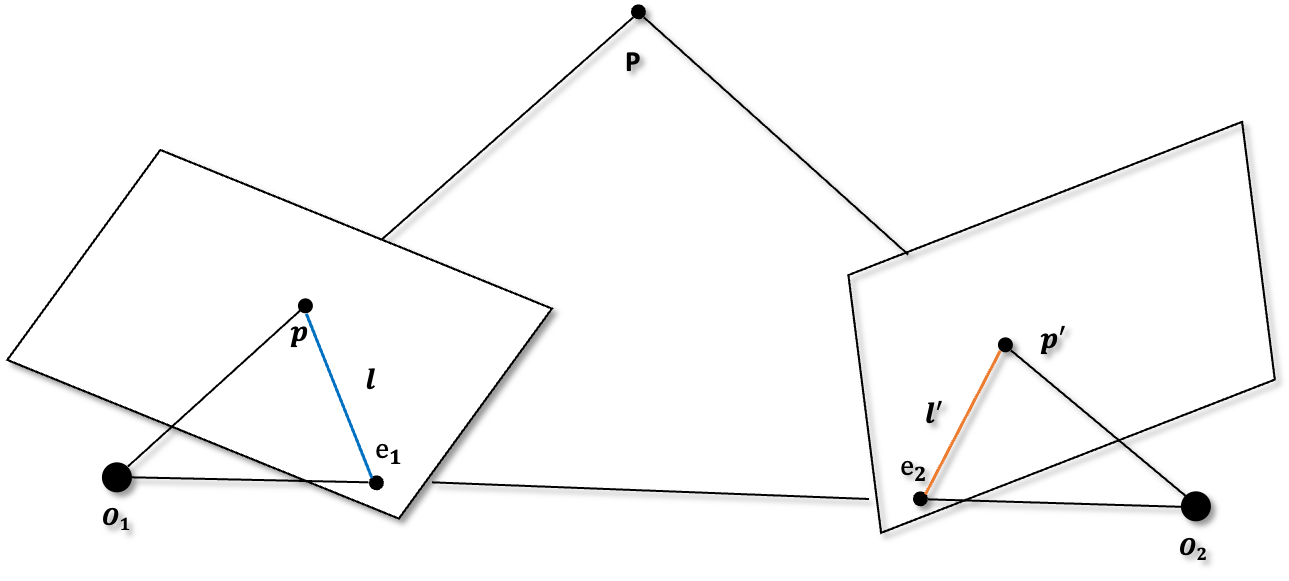
\includegraphics[width=0.8\textwidth]{images/base_matrix.png}
		\end{center}
		\caption{两图像之间的极几何约束,$O_1,O_2$为相机\textbf{光心},$O_1O_2$为\textbf{基线},$p,p^{\prime}$为$P$在两个像素平面的像,$e_1,e_2$为\textbf{极点},$l,l^{\prime}$为\textbf{极线}}
	\end{figure}

	\begin{align}
		&{p^{\prime}}^T \mathbf{F} p = 0 \\\label{f_constrain}
		&\mathbf{F} = {K^{\prime}}^{-T} [T{}]_{\times} RK^{-1} 
	\end{align}

	概念说明,
	\begin{itemize}
		\item 世界坐标系选为第一个相机坐标系
		\item $K,K^{\prime}$是两个相机的内参矩阵
		\item $R,T$是第二个相机相对第一个相机的旋转和平移
		\item $[T]_{\times}$是$T$张成的反称矩阵,秩为$2$,因此$F$的秩也为$2$
		\item $e,e^\prime$为对应像平面极点
	\end{itemize}

	$e^\prime$是$e$的投影,所以,
	$$
		e^\prime =K^\prime T
	$$

	因为$p^{\prime}$在极线$l^{\prime}$上,所以${{p^{\prime}}^Tl^{\prime} = 0}$,结合(\ref{f_constrain})可知,

	\begin{align*}
		l^{\prime} = Fp,\quad 
		l = F^Tp^\prime
	\end{align*}

	基础矩阵描述了点之间的约束关系,非一一对应关系,一个点对应到目标平面上的一条极线。\\

	极点$e^\prime$在极线$l^\prime$上,所以对任意$p$,
	$$
		{e^\prime}^T l^\prime = 0 \Rightarrow {e^\prime}^TFp=0 \Rightarrow p^T F^T e^\prime = 0
	$$

	因为$p$的任意性,可知

	$$
		{e^\prime}^T F = 0, Fe = 0
	$$

	基础矩阵刻画了点与极线的一一对应关系,沿着极线搜索$p$的像,会大幅缩小搜索范围。\\

	根据(\ref{inver_m_p}),可得到$F$的另一表达式,
	\begin{align*}
		F &= {K^{\prime}}^{-T}[T]_{\times}RK^{-1} \\
		  &= -{K^{\prime}}^{-T}[T]_{\times}^T RK^{-1}\\
		  &= -\left(
			[T]_{\times} {K^{\prime}}^{-1}
		\right)^T RK^{-1}\\
		  &=-\left(
			{K^{\prime}}^T \left[ K^\prime T\right]_{\times}
		\right)^T RK^{-1}\\
		&= [e^\prime]_{\times}K^{\prime} R K^{-1}
	\end{align*}	

	\begin{equation}
		F =  {K^{\prime}}^{-T} [T{}]_{\times} RK^{-1}  = [e^\prime]_{\times}K^{\prime} R K^{-1}\label{new_F_matrix}
	\end{equation}
	
	都是常用表达式。接下来通过两种方法确定$p^\prime,p$之间的表示关系,

	\subsection*{代数法}

		相机投影以及各种反投影虽然不一定构成射影变换,但一定是线性变换,所以$p^\prime$与$p$存在如下关系,
		$$
			p^\prime = \mathbf{A}p + \mathbf{b}
		$$

		只要确定$\mathbf{A},\mathbf{b}$即可。
		$$
			{p^\prime}^T\cdot\left(p^\prime \times \mathbf{b}\right)  = 0 \Rightarrow {p^\prime}^T\left(\mathbf{A}p\times \mathbf{b}\right) = 0 \Rightarrow {p^\prime}^T[\mathbf{b}]_{\times} \mathbf{A}p = 0
		$$

		对比基础矩阵约束可知, 
		$$ 
			F = [\mathbf{b}]_{\times} \mathbf{A} 
		$$

		而,
		$$
			F^T \mathbf{b} = -\mathbf{A}^T[\mathbf{b}_{\times}]\mathbf{b} = 0 \Rightarrow \mathbf{b} = e^{\prime}
		$$

		所以,
		$$
			F = [e^\prime]_{\times} \mathbf{A} 
		$$

		结合(\ref{new_F_matrix})可知

		$$
			A = K^{\prime} R K^{-1}
		$$

		因此,
		$$
			p^\prime  =  K^{\prime}\left(RK^{-1} p + T\right)
		$$

		从这个对应关系看出,$p^\prime,p$之间一般不服从射影变换。

	\subsection*{几何法}
		
		将$p$反投影回世界坐标系,再投影到第二个相机的像素平面的$p^\prime$,根据(\ref{inverse_proj}),

		\begin{align}
			p^{\prime}(d) &= K^{\prime}[R\quad T]
			\begin{bmatrix}
				dK^{-1}p\\
				1
			\end{bmatrix}\\
			&= K^{\prime}\left(dRK^{-1}p + T\right)\label{f_inverse}
		\end{align}

		当$d$变动时$p^{\prime}(d)$实际就是上面讨论的极线。\\

		在齐次坐标下,尺度$d$是无关紧要的,几何法代数法结论一致的,过程更容易理解。\\

		几何法没有利用基础矩阵,需要验证结果满足基础矩阵约束,${p^{\prime}}^T F p = 0$
		\begin{align*}
			&{p^{\prime}}^T F p = 0\\
			&\quad\quad\Downarrow\\
			&\left[
				K^{\prime}\left(dRK^{-1}p + T\right)
			\right]^{T} 
			{K^{\prime}}^{-T} [T]_{\times} R K^{-1}p = 0\\
			&\quad\quad\Downarrow\\
			&\left(
				dRK^{-1}p + T
			\right)^{T} {K^{\prime}}^T {K^{\prime}}^{-T} [T]_{\times} R K^{-1}p = 0\\
			&\quad\quad\Downarrow\\
			&\left(dp^TK^{-T}R^T + T^T\right) [T]_{\times} R K^{-1}p = 0\\
			&\quad\quad\Downarrow\\
			&p^TK^{-T}R^T [T]_{\times} R K^{-1}p = 0\\
			&\quad\quad\Downarrow \\
			&p^T\mathbf{A}p = 0	\quad\left(\mathbf{A}= K^{-T} R^T [T]_{\times} R K^{-1},\mathbf{A} = -\mathbf{A}^T\right)
		\end{align*}

			最后一步是因为对任意反称矩阵$\mathbf{A}$都满足$ p^T \mathbf{A} p = 0 $。

	\subsection*{工程实现}
		之所有讨论代数法和几何法,是因为在偏理论的文章中会直接给出代数结果,而在偏工程的文献中又会根据几何变换给出一个结果,
		我们需要确保,从不同文献来的结果本质是一样的。\\

		在实际计算时,通过增广的投影矩阵表示更为方便,
		\begin{equation}
			N_d= M^{\prime}M^{-1} = \begin{bmatrix}
				dK^\prime R K^{-1} \quad& K^\prime T\\
				0\quad& 1\quad
			\end{bmatrix}\label{extend_f}		
		\end{equation}

		从$N_d$中截取出左上角$3\times 3$的矩阵便是旋转矩阵,右上角$3\times 1$的向量是平移向量,这在各种工具中非常容易实现。

\section{单应变换}

	如前所述,如果拍摄场景是一张平面,(\ref{f_inverse})可表示为射影变换,我们看看这个结论怎么来的。\\

	设场景平面法向量为$\mathbf{n}$,到原点距离为$d$,则平面方程为,
	$$
		\mathbf{n}^T P = d
	$$

	令$\mathbf{n}_d = \mathbf{n}/d$,场景平面可表示为$\mathbf{n}_d^T P = 1$。\\

	场景平面距离为$d$,像素点$p$反投影为$dK^{-1}p$,

	\begin{align*}
		p^{\prime}(d) &= K^{\prime}\left(dRK^{-1}p + T\right)\\
		&= K^{\prime}\left(dRK^{-1}p + T\mathbf{n}_d^T P\right)\\
		&= K^{\prime}\left(dRK^{-1}p + T\mathbf{n}_d^TdK^{-1}p\right)\\
		&= dK^{\prime}\left(R + T\mathbf{n}_d^T\right)K^{-1}p\\
		&= Hp
	\end{align*}

	这里的关键是第二步,代入场景平面方程,把$p$给分离了出来。\\

	$K^\prime$是齐次矩阵,与$dK^\prime$等价。

	\begin{equation}
		H= K^{\prime}\left(R + T\mathbf{n}_d^T\right)K^{-1} \label{homograph_matrix}
	\end{equation}

	称为\textbf{单应矩阵},因此射影变换也称为单应变换。$p,p^{\prime}$依然服从基础矩阵的约束,(\ref{extend_f})式的增广表示也包含了单应变换这一特殊情况。\\

	基础矩阵只能得到点与极线的对应关系,而单应变换能进一步得到点之间的对应关系。\\

	在MVSNet中,只知道两个相机在世界坐标系的旋转和平移$R_1,t_1,R_2, t_2$,相对旋转$R$和平移$t$为,

	$$
		R = R_2R_1^{-1},\quad 
		t = t_2 - R_2R_1^{-1}t_1
	$$

	(\ref{homograph_matrix})用世界坐标系可表示为,

	\begin{align}
		H &= K_2 \left(R_2R_1^{-1} +\left(t_2 - R_2R_1^{-1}t_1\right) \mathbf{n}_d^T\right) K_1^{-1} \label{new_homograph_matrix}
	\end{align}	

	原论文中的公式是错误的,这是正确版本。\\

	因为增广表示蕴含了单应变换,所以这个复杂的式子在编程中根本用不到。

\section{SfM}
	\definition{SfM问题} 也称为\textbf{欧式结构恢复问题},已知$m$张图片和对应的相机内参矩阵$K_i(i=1,\cdots,m)$,求解:
	\begin{itemize}
		\item \textbf{Structure}:$n$个三维点$X_j(j=1,\cdots\,n)$的坐标
		\item \textbf{Motion}:$m$个相机的外参数$R_i,T_i(i=1,\cdots,m)$
	\end{itemize}		
	
	如果没有额外信息,无法恢复出场景的绝对坐标(经纬度)、朝向及尺度,恢复的最好结果是与真实场景之间差一个相似变换;\\

	比如,如果知道场景中某两点之间的真实距离,则可恢复出场景的尺度,但依然无法确定绝对坐标和朝向。

	\subsection{两视图重建}

	考虑两张图片的场景,根据(\ref{base_matrix}),只要能估计出基础矩阵$F$,就可能估计出$R,T$,
	$$
		F = {K^{\prime}}^T [T_{\times}] RK^{-1}
	$$

	根据基础矩阵约束,$p=(u,v,1)^T,p^{\prime} = (u^{\prime}, v^{\prime},1)$
	$$
		{p^{\prime}}^T F p = 0 \Rightarrow (u^{\prime}, v^{\prime},1)
		\begin{bmatrix}
			F_{11}\quad& F_{12}\quad& F_{13}\\
			F_{21}\quad& F_{22}\quad& F_{23}\\
			F_{31}\quad& F_{32}\quad& F_{33}\\
		\end{bmatrix}
		(u,v,1)^T = 0
	$$
	展开可得,

	$$
		\left(uu^{\prime}, vu^{\prime}, u^{\prime}, uv^{\prime},vv^{\prime},v^{\prime},u,v,1\right)
		\begin{bmatrix*}
			F_{11}\\
			F_{12}\\
			F_{13}\\
			F_{21}\\
			F_{22}\\
			F_{23}\\
			F_{31}\\
			F_{31}\\
			F_{33}
		\end{bmatrix*} = 0
	$$

	在不考虑尺度的情况下,$F$矩阵有8个未知数,因此至少需要8对点才能确定$F$,实际上会用大于8对点,求一个最小二乘解。\\

	$F$的秩为2,最小二乘解得到的矩阵秩一般为3,需要做一次SVD分解,置最小特征值为0,来得到$F$。

	\subsubsection*{解的存在性}
		是不是任意的8对点一定能求解出$F$呢?如果8个方程中部分线性相关,会导致方程的数量少于未知数的数量,从而没有唯一解。\\

		比如场景是一张平面,$P_1,P_2,P_3$是平面上不共线的三点,对应像素平面$p_1,p_2,p_3$三点;对应第二个像素平面$p^\prime_1,p^\prime_2,p^\prime_2$;

		平面上任意点$P$可表示为三点的线性组合,$P=\alpha P_1 + \beta P_2 + \gamma P_3$,$P$的投影为,
		
		\begin{align*}
			p &= K\left(\alpha P_1 + \beta P_2 + \gamma P_3\right)\\
				&= \alpha KP_1 + \beta K P_2 + \gamma KP_3\\
				&= p_1 + p_2 + p_3
		\end{align*}

		场景平面存在单应变换,
		$$
			p^\prime = Hp = Hp_1 + Hp_2 + Hp_3 = p^\prime_1+p^\prime_2+p^\prime_3
		$$

		也就是说$(p_1 + p_2 + p_3,p^\prime_1+p^\prime_2+p^\prime_3)$构成点对,这个点对没有增加新点,是一个冗余方程,此时基础矩阵没有唯一解。\\

		实际上要使得线性无关的方程数量至少为8,方程才有唯一解。

		\begin{itemize}
			\item 没有解的时候基础矩阵怎么表示?
			\item 我们怎么知道在给定的点对中,有多少个线性无关的方程呢?
		\end{itemize}

		第一个问题,在单应变换的情况下,需要求解单应矩阵,基础矩阵的元素也都包含在单应矩阵中;\\

		第二个问题,实际上会用一个粗暴的办法,先用基础矩阵求解一次,再用单应矩阵求解一次,哪个效果好用哪个,不再去探讨解的存在性。

	\subsubsection*{确定对应点对}
		怎么确定两张图像的对应点对$p,p^{\prime}$?可以用传统的SIFT特征匹配,也可以用深度学习的方法,这里就不再详细介绍。\\

	
	注意这里世界坐标系选择为第一个相机的坐标系,因此只有第二个相机的$R,T$需要求解,得到基础矩阵$R,T$后,根据投影关系,
	$$
		p^{\prime} = K^{\prime}[R\quad T]\begin{bmatrix}
			P\\
			1
		\end{bmatrix}
	$$

	可计算出空间点$P$的3D坐标,如前所述,这个坐标是在第一个相机坐标系下的坐标,并且重建出的目标会跟真实大小相差一个尺度。

	\subsection{多视图重建}
		在多视图重建场景,有多张图片,多个相机内参矩阵,求解SfM问题常用\textbf{增量法},具体来说包括几个步骤,
	
	\begin{itemize}
		\item 相机之间通过两视图方法两两求解$F_{ij}$
		\item 从一对相机开始,不断加入其他相机,这样重建的点会越来越多
		\item 持续加入相机会累积误差,所以通过\textbf{捆绑调整}(Bundle Adjustment)来做一个整体调整
	\end{itemize}

	其中细节和技巧非常多,具体请参考鲁鹏老师的课程\footnote{\url{https://www.bilibili.com/video/BV1Ss4y197CU}}(多视图重建一节)。\\

	这里要说的是这个\textbf{捆绑调整}方法,本质就是最小化投影误差,
	$$
		E(M,X) = \sum_{i=1}^m \sum_{j=1}^n D\left(x_{ij}, M_iX_j\right)^2
	$$

	\begin{figure}[H]
		\begin{center}
			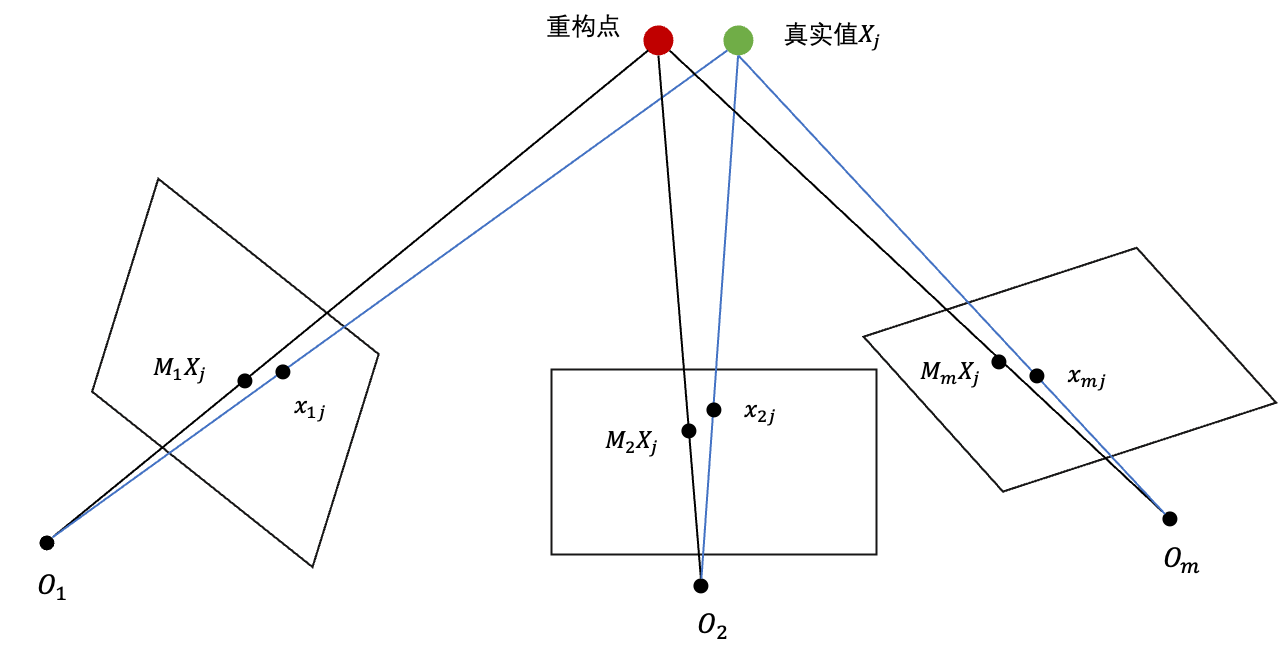
\includegraphics[width=\textwidth]{images/ba.png}
		\end{center}
		\caption{BA重投影误差}
	\end{figure}

	BA是借助了一个$L_2$距离来做全局优化,实际这个距离选择在机器学习里面非常的多。经过一番操作,我们得到一些3D点的坐标,也就是场景点云。\\

	不是每张照片上的点都能得到一个深度信息,至少被两个相机看到,能构成$p,p^{\prime}$对的点才能计算出深度。拍摄照片时,相邻相机偏离角度不能太大,否则因为遮挡导致可匹配的点减少,影响重建效果。\\

	BA优势就是不需要所有的点都被所有的相机看到,每个相机只关注自己能看到点即可。

\section{MVSNet}

	不同于传统的SfM估计一次优化能得到整个场景的点云,MVSNet\footnote{\url{https://arxiv.org/abs/1804.02505}}只是推断每张图片的深度信息,通过后处理,把多张图片的深度,拼成场景点云。\\

	主要思路是通过2张目标图来协助推断参考图的深度值,

	\begin{enumerate}
		\item 把参考相机(第一个相机)像素平面的坐标,通过192个尺度反投影到相机坐标系;然后通过单应矩阵变换到目标相机的像素坐标系。

		\small\textit{ 注意,这里的变换对象是参考相机的$120 \times 160$像素平面坐标,而非论文说的参考图像的特征图;}

		经过这步操作,可在目标相机的像素平面上形成192个$120 \times 160$的新的像素坐标值。

		\item 把投影得到的像素坐标值与目标图像的特征图结合,得到192个目标特征图

		\small\textit{把192个特征图按深度叠在一起,形成一个$192 \times 120 \times 160 \times 32$的特征图,称为\textbf{Feature Volume}}

		\item 把多个(文中为2个)目标\textbf{Feature Volume}连同参考图像的特征图一起,计算一个方差,得到的结果称为\textbf{Cost Volume},随后在\textbf{Cost Volume}上回归参考图像的深度值

		\small\textit{注意,此时才用到参考图像的特征图}
	\end{enumerate}

	\begin{figure}[H]
		\begin{center}
			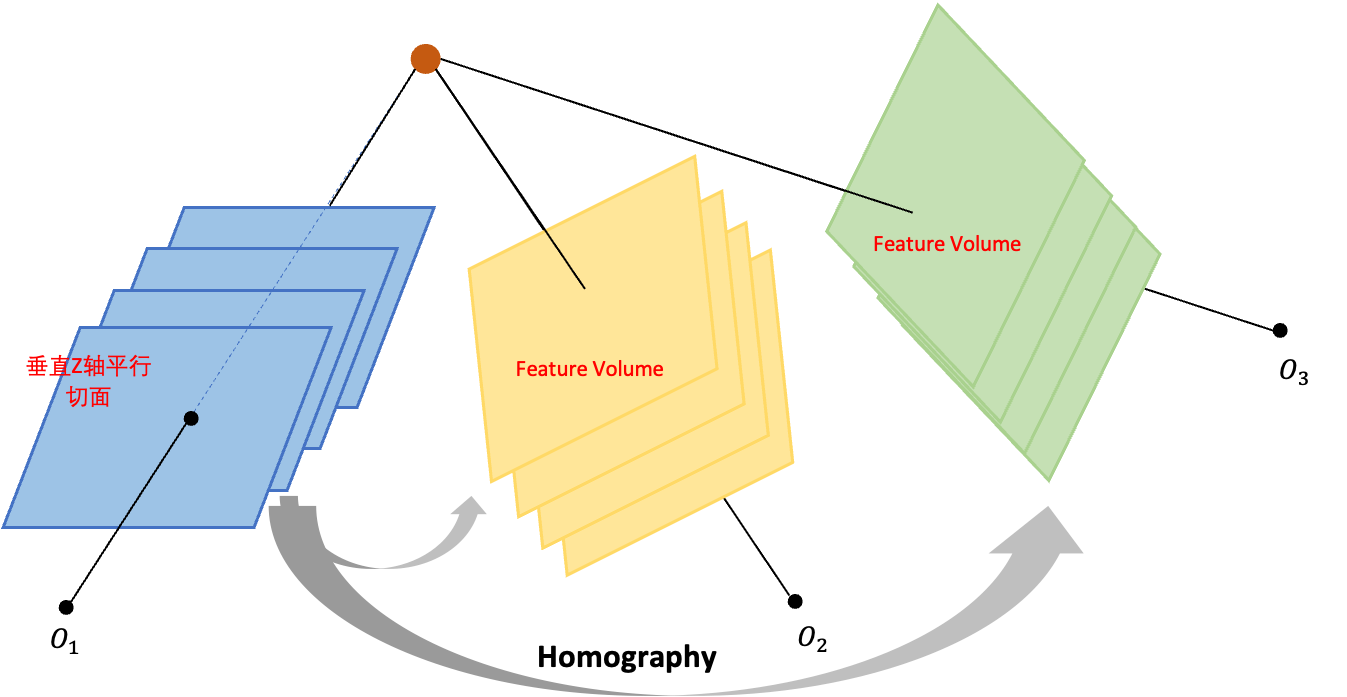
\includegraphics[width=\textwidth]{images/fronto.png}
		\end{center}
		\caption{相机1将场景按深度切片称为\textbf{Fronto parallel},分别投影到相机2,3像素平面,形成\textbf{Feature Volume}}
	\end{figure}

\subsection{目标相机的作用}

	目标相机对预测参考图像的深度有什么帮助?我是这么认为的,因为世界坐标系选为参考相机的坐标系,如果参考图像上有一个点深度为$d$,那么其他相机看到这个点深度也应该为$d$,也就是用目标图像的特征预测出的深度也应该为$d$。\\

	因此,如果一个点的深度在各个相机下预测正确,那么方差就会很小,否则方差会变大,这是作者认为\textbf{Cost Volume}有作用的原因。\\

	把\textbf{Feature Volume}的平均作为回归目标也是可行的,但作者在消融实验提到效果不如方差,这里是个玄学。\\

	提升目标图片数量,预测效果也会提升,作者实验过5张图片效果好于2张。能提升预测效果的图片是那些与目标相机姿态差距不是很大的图片,所以这个数量也是有上限的。

\subsection{单应变换的作用}
	MVSNet工作重点便是单应变换,主要体现在:
	\begin{itemize}
		\item 通过单应变换把场景切面变换到目标相机像素坐标系
		\item 单应变换可求导,使得变换过程可训练
	\end{itemize}

	然而,变换切面通过增广矩阵的逆变换即可,矩阵变换本身可求导,顺便包含了第二点。\\

	虽然全文都在介绍单应矩阵,实现实际完全不需要这个概念,更不需要那些复杂的推导,是不是有点讽刺!\\

	需要考虑下面两个问题,对单应变换的影响,
	\begin{itemize}
		\item 不同深度的切面通过单应变换产生的像素值会有多大的差异?
		\item 单应变换产生的新坐标如何跟目标特征图结合生成新的特征图?
	\end{itemize}

	\subsubsection*{深度对像素坐标的影响}
	对第一个问题,单应矩阵$H$可以简化为,

	\begin{align*}
		H_d= K^{\prime}\left(R + T\mathbf{n}_d^T\right)K^{-1} &= \mathbf{A} +\frac{1}{d}\mathbf{B}\\
		&= \begin{bmatrix}
			\mathbf{A}_1 + \frac{1}{d}\mathbf{B}_1\\
			\mathbf{A}_2 + \frac{1}{d}\mathbf{B}_3\\
			\mathbf{A}_3 + \frac{1}{d}\mathbf{B}_4
		\end{bmatrix}
	\end{align*}

	$\mathbf{A}=K^\prime R K^{-1},\mathbf{B}=K^{\prime}T\mathbf{n}^TK^{-1}$,只有$d$是变量,
	$$
		p^\prime(d) = H_d p = \begin{bmatrix}
			\left(\mathbf{A}_1 + \frac{1}{d}\mathbf{B}_1\right)p\\
			\left(\mathbf{A}_2 + \frac{1}{d}\mathbf{B}_3\right)p\\
			\left(\mathbf{A}_3 + \frac{1}{d}\mathbf{B}_4\right)p
		\end{bmatrix}
	$$

	$p^\prime$的欧式坐标$p^\prime_e$为,
	$$
		p^\prime_e(d) = \left(
			\frac{\left(\mathbf{A}_1 + \frac{1}{d}\mathbf{B}_1\right)p}{\left(\mathbf{A}_3 + \frac{1}{d}\mathbf{B}_3\right)p},
			\frac{\left(\mathbf{A}_2 + \frac{1}{d}\mathbf{B}_3\right)p}{\left(\mathbf{A}_3 + \frac{1}{d}\mathbf{B}_3\right)p}
		\right)^T
	$$

	$$
		p^\prime_e(\infty) = \lim_{d\rightarrow \infty}p^\prime_e(d) = \left(
			\frac{\mathbf{A}_1p}{\mathbf{A}_3p},
			\frac{\mathbf{A}_2p}{\mathbf{A}_3p}
		\right)^T
	$$

	$$
		p^\prime_e(0) = \lim_{d\rightarrow 0}p^\prime_e(d) = \left(
			\frac{\mathbf{B}_1p}{\mathbf{B}_3p},
			\frac{\mathbf{B}_2p}{\mathbf{B}_3p}
		\right)^T
	$$	

	深度$d$的确影响投影的$u,v$坐标,且输出在$p^\prime_e(0)$和$p^\prime_e(\infty)$之间。\\

	但因为在两端存在极限,所以$d$在一定的区间内变化,对$u,v$才能有显著的影响,
	
	\subsubsection*{变换特征映射}
		现在考虑第二个问题,参考相机和目标相机像素平面分辨率为$120 \times 160$,超出这个区间的变换坐标怎么处理?\\

		MVSNet的是根据最大坐标值,$u^\prime = u/119, v^\prime = v/159$(坐标从0开始)后变换到$[-1,1]$,对超出此区间的坐标一律忽略。\\

		目标特征图的左上角对应$(-1,-1)$,右下角对应$(1,1)$,根据$(u^\prime, v^\prime)$的值查找特征图上对应的点(连续值),并根据周围四个坐标(离散值)做双线性插值计算具体对应值。\\

		显然,考相机和目标相机的分辨率即使不同,也不影响这个插值过程。\\

		如果超出$(120,160)$的坐标都被忽略,是否会降低学习效果?\\

		这里实际隐含一个约束,要求两个相机应该能看到尽量多的共同点,这通过pair图像的选择策略来实现。

\subsection{实现细节}
	MVSNet将$1200 \times 1600$的原图下采样到$800 \time 600$,从中心crop出$512 \times 640$作为输入,经过特征提取后生成$128 \times 160 \times 32$的特征图。\\

	输出为参考图的深度值,GroundTruth也是参考图的深度值,均为$128 \times 160$。 处理分几个步骤,

	\begin{itemize}
		\item 每次输入3张图,一张为参考,2张目标,经过特征提取后,得到三个$128 \times 160 \times 32$的特征图
		
		\item 采用192个深度单位,通过单应变换将参考坐标变换到两个目标相机姿态下

			\textit{作者原始实现用了复杂的单应矩阵,非常繁琐;pytorch版本用了增广变换矩阵,非常简洁}

		\item 根据坐标变换得到两个$192 \times 128 \times 160 \times 32$的特征图,如上节描述

			\textit{按深度方向,从425mm到935mm,按2mm间隔离散成192个像平面}

		\item 连同参考特征图一起,计算三个\textbf{Feauture Volume}的方差,得到\textbf{Cost Volume};进行3D卷积,通过softmax沿着深度方向作概率归一化,结果为\textbf{Probability Volume},维度为$192 \times 128 \times 160$

		\item 沿\textbf{Probability Volume}深度方向计算深度期望值,得到维度为$128 \times 160$的深度特征图,
			$$
				D = \sum_{d = d_{min}}^{d_{max}} d \times \mathbf{P}(d)
			$$

			论文中提到,这一步实际想对\textbf{Probability Volume}作一个$\arg\max$操作,选出当前位置最可能的深度值,但是$\arg\max$无法求导,无法进行梯度回传,所以用soft $\arg\max$(原文说成是soft $\arg\min$)。

			\textit{所谓soft $\arg\max$实际就是利用了$softmax$逼近$\arg\max$的特性,以此来代替$\arg\max$\footnote{\url{https://en.wikipedia.org/wiki/Softmax_function}}}

		\item 通过$L_1$回归参考图的深度值;这里只有参考图的深度值为GroundTruth,src图的深度值未使用。
	\end{itemize}

	在增量SfM方法中,一次考虑所有图像,通过反投影距离进行优化,得到整个场景的点云;但在具体实现中,至少被三个相机看到的点,才能重建出点云;\\

	MVSNet中,训练的时候只是用了3张图片,但可以推断出参考图像上所有点的深度信息;在后处理时需要把图片两两输入,构建整个场景的点云。\\

	SfM的依赖图像之间的对应点对,具体会通过SIFT特征或深度学习的方法去构建对应关系;这一步实际也会引入很多匹配噪音,尤其对一些纹理较少的图像,能计算出的匹配点较少。\\

	MVSNet没有这一步处理,对应关系已经隐含在深度预测中,能匹配的点对,看到的深度也应该一样。\\

	事实证明,通过隐式特征构建对应关系,远远好于在RGB空间用显式特征构建对应关系。

\subsection{问题\&改进}
	为什么要将场景切成192片,作单应变换去构建Cost,而不是直接通过基础矩阵变换构建Cost?\\

	单应变换是传统处理常用的手段,这个文章发表比较早,受传统MVS影响比较大,可能当时还没有建立端到端的思路,或者是端到端没做出效果。\\

	切片思路得假设目标场景最大最小距离,切片多了影响计算性能,并且有很多无意义的切片;切片少了又影响精度,对此"Cascade Cost Volume for High-Resolution Multi-View Stereo and Stereo Matching"\footnote{\url{https://arxiv.org/abs/1912.06378}}这个文章专门提了一些切片的优化方法,后面我们再细说。

\section{训练集结构}
	
	\subsection*{DTU数据集} 
		mvsnet用的是DTU数据集,DTU数据集通过移动的机械臂在$49$或$64$个位置,用$7$种光照,通过结构光扫描了$124$个场景,生成$1200 \times 1600$像素的图片及对应的点云信息。\\

		因此,每个场景有$49 * 7 = 343$张照片,整体数据集包含$42532$张照片及对应的点云信息。因为机械臂移动受到严格控制,所以每张图片都有对应的高精度相机参数。\\

		mvsnet训练集用了$79$个场景,共计$27097$张图片;测试集用了$22$个场景,共计$7546$张图片。
	
	\subsection*{深度信息}
		MVSNet的输入的是每个点的深度,通过泊松表面重建,将DTU数据集的点云转变为mesh,计算出每个像素点对应的深度信息。

	\subsection*{数据集结构}
		\begin{itemize}
			\item mvs{\_}training$\slash$dtu$\slash$Cameras$\slash$pair.txt 记录了$49$个位置,每个位置的照片与其他$10$张照片的匹配程度;注意这个pair内容与场景无关,仅与相机位置有关。因为相机位置受到精准控制,所以通过空间关系可以描述出位置之间的差异。

			\item mvs{\_}training$\slash$dtu$\slash$Cameras{\_}train$\slash$000000\{YY\}{\_}cam.txt 存放相机内外参数及尺度缩放信息

			\item mvs{\_}training$\slash$dtu$\slash$Rectified$\slash$scan\{XX\}{\_}train 训练样本,XX为场景编号
				\begin{itemize}
					\item rect{\_}0\{YY\}{\_}\{Z\}{\_}r5000 为场景scanXX对应的图片,YY为相机位置编号$ 1 \sim 49$,Z为光照强度编号$0 \sim 6$
				\end{itemize}

			\item mvs{\_}training$\slash$dtu$\slash$Depths$\slash$scan\{XX\}{\_}train$\slash$
				\begin{itemize}
					\item depth{\_} map{\_}00\{YY\}.pfm 场景scanXX对应相机位置YY($0 \sim 48$)的深度图,格式为pfm
					\item depth{\_} map{\_}00\{YY\}.png 深度图的可视化
				\end{itemize}
			
		\end{itemize}	